% Options for packages loaded elsewhere
\PassOptionsToPackage{unicode}{hyperref}
\PassOptionsToPackage{hyphens}{url}
\PassOptionsToPackage{dvipsnames,svgnames,x11names}{xcolor}
%
\documentclass[
  ignorenonframetext,
]{beamer}
\usepackage{pgfpages}
\setbeamertemplate{caption}[numbered]
\setbeamertemplate{caption label separator}{: }
\setbeamercolor{caption name}{fg=normal text.fg}
\beamertemplatenavigationsymbolsempty
% Prevent slide breaks in the middle of a paragraph
\widowpenalties 1 10000
\raggedbottom

\usepackage{amsmath,amssymb}
\usepackage{iftex}
\ifPDFTeX
  \usepackage[T1]{fontenc}
  \usepackage[utf8]{inputenc}
  \usepackage{textcomp} % provide euro and other symbols
\else % if luatex or xetex
  \usepackage{unicode-math}
  \defaultfontfeatures{Scale=MatchLowercase}
  \defaultfontfeatures[\rmfamily]{Ligatures=TeX,Scale=1}
\fi
\usepackage{lmodern}
\usetheme[]{AnnArbor}
\usecolortheme{dolphin}
\usefonttheme{structurebold}
\ifPDFTeX\else  
    % xetex/luatex font selection
\fi
% Use upquote if available, for straight quotes in verbatim environments
\IfFileExists{upquote.sty}{\usepackage{upquote}}{}
\IfFileExists{microtype.sty}{% use microtype if available
  \usepackage[]{microtype}
  \UseMicrotypeSet[protrusion]{basicmath} % disable protrusion for tt fonts
}{}
\makeatletter
\@ifundefined{KOMAClassName}{% if non-KOMA class
  \IfFileExists{parskip.sty}{%
    \usepackage{parskip}
  }{% else
    \setlength{\parindent}{0pt}
    \setlength{\parskip}{6pt plus 2pt minus 1pt}}
}{% if KOMA class
  \KOMAoptions{parskip=half}}
\makeatother
\usepackage{xcolor}
\newif\ifbibliography
\setlength{\emergencystretch}{3em} % prevent overfull lines
\setcounter{secnumdepth}{-\maxdimen} % remove section numbering


\providecommand{\tightlist}{%
  \setlength{\itemsep}{0pt}\setlength{\parskip}{0pt}}\usepackage{longtable,booktabs,array}
\usepackage{calc} % for calculating minipage widths
\usepackage{caption}
% Make caption package work with longtable
\makeatletter
\def\fnum@table{\tablename~\thetable}
\makeatother
\usepackage{graphicx}
\makeatletter
\def\maxwidth{\ifdim\Gin@nat@width>\linewidth\linewidth\else\Gin@nat@width\fi}
\def\maxheight{\ifdim\Gin@nat@height>\textheight\textheight\else\Gin@nat@height\fi}
\makeatother
% Scale images if necessary, so that they will not overflow the page
% margins by default, and it is still possible to overwrite the defaults
% using explicit options in \includegraphics[width, height, ...]{}
\setkeys{Gin}{width=\maxwidth,height=\maxheight,keepaspectratio}
% Set default figure placement to htbp
\makeatletter
\def\fps@figure{htbp}
\makeatother
% definitions for citeproc citations
\NewDocumentCommand\citeproctext{}{}
\NewDocumentCommand\citeproc{mm}{%
  \begingroup\def\citeproctext{#2}\cite{#1}\endgroup}
\makeatletter
 % allow citations to break across lines
 \let\@cite@ofmt\@firstofone
 % avoid brackets around text for \cite:
 \def\@biblabel#1{}
 \def\@cite#1#2{{#1\if@tempswa , #2\fi}}
\makeatother
\newlength{\cslhangindent}
\setlength{\cslhangindent}{1.5em}
\newlength{\csllabelwidth}
\setlength{\csllabelwidth}{3em}
\newenvironment{CSLReferences}[2] % #1 hanging-indent, #2 entry-spacing
 {\begin{list}{}{%
  \setlength{\itemindent}{0pt}
  \setlength{\leftmargin}{0pt}
  \setlength{\parsep}{0pt}
  % turn on hanging indent if param 1 is 1
  \ifodd #1
   \setlength{\leftmargin}{\cslhangindent}
   \setlength{\itemindent}{-1\cslhangindent}
  \fi
  % set entry spacing
  \setlength{\itemsep}{#2\baselineskip}}}
 {\end{list}}
\usepackage{calc}
\newcommand{\CSLBlock}[1]{\hfill\break\parbox[t]{\linewidth}{\strut\ignorespaces#1\strut}}
\newcommand{\CSLLeftMargin}[1]{\parbox[t]{\csllabelwidth}{\strut#1\strut}}
\newcommand{\CSLRightInline}[1]{\parbox[t]{\linewidth - \csllabelwidth}{\strut#1\strut}}
\newcommand{\CSLIndent}[1]{\hspace{\cslhangindent}#1}


% logo
\titlegraphic{
\includegraphics[width=4cm]{000_logos/logo-blue-vertical}}
\logo{\ifnum\thepage>1
\includegraphics[width=0.5cm]{000_logos/logo-blue-vertical}\fi}

% UMNG: Manual de image institucional

% Colors

% Umng
\definecolor{yellow}{HTML}{fdc600}
\definecolor{red}{HTML}{ee2a24}

% Estudios a Distancia
\definecolor{blue1}{HTML}{12245b}
\definecolor{blue2}{HTML}{767ca6}
\definecolor{blue3}{HTML}{cad2ec}

% Modify items
\setbeamercolor{palette primary}{bg=blue3}
\setbeamercolor{palette tertiary}{bg=blue1}
\setbeamercolor{frametitle}{bg=yellow}

% Hyperlinks
\hypersetup{
  linkcolor=red,
  citecolor=red
}

\makeatletter
\@ifpackageloaded{caption}{}{\usepackage{caption}}
\AtBeginDocument{%
\ifdefined\contentsname
  \renewcommand*\contentsname{Table of contents}
\else
  \newcommand\contentsname{Table of contents}
\fi
\ifdefined\listfigurename
  \renewcommand*\listfigurename{List of Figures}
\else
  \newcommand\listfigurename{List of Figures}
\fi
\ifdefined\listtablename
  \renewcommand*\listtablename{List of Tables}
\else
  \newcommand\listtablename{List of Tables}
\fi
\ifdefined\figurename
  \renewcommand*\figurename{Figure}
\else
  \newcommand\figurename{Figure}
\fi
\ifdefined\tablename
  \renewcommand*\tablename{Table}
\else
  \newcommand\tablename{Table}
\fi
}
\@ifpackageloaded{float}{}{\usepackage{float}}
\floatstyle{ruled}
\@ifundefined{c@chapter}{\newfloat{codelisting}{h}{lop}}{\newfloat{codelisting}{h}{lop}[chapter]}
\floatname{codelisting}{Listing}
\newcommand*\listoflistings{\listof{codelisting}{List of Listings}}
\makeatother
\makeatletter
\makeatother
\makeatletter
\@ifpackageloaded{caption}{}{\usepackage{caption}}
\@ifpackageloaded{subcaption}{}{\usepackage{subcaption}}
\makeatother

\ifLuaTeX
\usepackage[bidi=basic]{babel}
\else
\usepackage[bidi=default]{babel}
\fi
\babelprovide[main,import]{english}
% get rid of language-specific shorthands (see #6817):
\let\LanguageShortHands\languageshorthands
\def\languageshorthands#1{}
\ifLuaTeX
  \usepackage{selnolig}  % disable illegal ligatures
\fi
\usepackage{bookmark}

\IfFileExists{xurl.sty}{\usepackage{xurl}}{} % add URL line breaks if available
\urlstyle{same} % disable monospaced font for URLs
\hypersetup{
  pdftitle={External sector II},
  pdfauthor={Luis Francisco Gómez López},
  pdflang={en},
  colorlinks=true,
  linkcolor={Maroon},
  filecolor={Maroon},
  citecolor={Blue},
  urlcolor={Blue},
  pdfcreator={LaTeX via pandoc}}


\title{External sector II}
\author{Luis Francisco Gómez López}
\date{2024-07-16}
\institute{FAEDIS}

\begin{document}
\frame{\titlepage}

\renewcommand*\contentsname{Table of contents}
\begin{frame}[allowframebreaks]
  \frametitle{Table of contents}
  \tableofcontents[hideallsubsections]
\end{frame}

\section{Please Read Me}\label{please-read-me}

\begin{frame}{}
\phantomsection\label{section}
\begin{itemize}
\item
  Check the message \textbf{Welcome greeting} published in the News
  Bulletin Board.
\item
  Dear student please edit your profile uploading a photo where your
  face is clearly visible.
\item
  The purpose of the virtual meetings is to answer questions and not to
  make a summary of the study material.
\item
  This presentation is based on
  (\citeproc{ref-cardenas_introduccion_2020}{Cardenas 2020, chap. 5})
\end{itemize}
\end{frame}

\section{Purpose}\label{purpose}

\begin{frame}{}
\phantomsection\label{section-1}
Explain the composition and determinants of Colombian foreign trade
\end{frame}

\section{The concept of comparative
advantage}\label{the-concept-of-comparative-advantage}

\begin{frame}{}
\phantomsection\label{section-2}
\begin{itemize}
\item
  \textbf{Absolute advantage}: the ability of a party (individual,
  company, country) to produce a product more efficiently than any other
  party

  \begin{itemize}
  \item
    A party should concentrate in producing a good in which it has an
    absolute advantage
  \item
    ¿What happend when you don't have an absolute advantage?
  \end{itemize}
\item
  \textbf{Comparative advantage}: the ability of a party (individual,
  company, country) to produce a product at a lower relative opportunity
  cost

  \begin{itemize}
  \tightlist
  \item
    Under certain conditions, even if a party doesn't have an
    \textbf{absolute advantage}, trade with other agent can be benefical
    for both of them
  \end{itemize}
\end{itemize}
\end{frame}

\begin{frame}{}
\phantomsection\label{section-3}
\begin{itemize}
\item
  Example of gains of trade using the concept of \textbf{comparative
  advantage} (\citeproc{ref-ridley_when_2010}{Ridley 2010})

  \begin{itemize}
  \item
    \textbf{Agent 1} produce 1 spear in 4 hours and 1 axe in 3 hours.

    \begin{itemize}
    \tightlist
    \item
      To produce both products \textbf{agent 1} will need to allocate 7
      hours
    \end{itemize}
  \item
    \textbf{Agent 2} produce 1 spear in 1 hour and 1 axe in 2 hours.

    \begin{itemize}
    \tightlist
    \item
      \textbf{Agent 2} has the absolute advantage in the prodution of
      spears and axes.
    \item
      To produce both products \textbf{agent 2} will need to allocate 3
      hours
    \end{itemize}
  \item
    ¿It will be benefical for agent 1 and 2 to trade? Yes!!!
    \textbf{Agent 1} can produce 2 axes in 6 hours and \textbf{agent 2}
    2 spears in 2 hours. Then they can trade 1 spear for 1 axe.

    \begin{itemize}
    \tightlist
    \item
      \textbf{Agent 1} has now 1 spear and 1 axe only working 6 hours.
    \item
      Furthermore \textbf{agent 2} has now 1 spear and 1 axe only
      working 2 hours.
    \item
      Each of them saves 1 hour of work in contrast with a situation in
      which they don't trade and produce themselves both products.
    \end{itemize}
  \end{itemize}
\end{itemize}
\end{frame}

\section{Volume of international
trade}\label{volume-of-international-trade}

\begin{frame}{}
\phantomsection\label{section-4}
\begin{figure}

\centering{

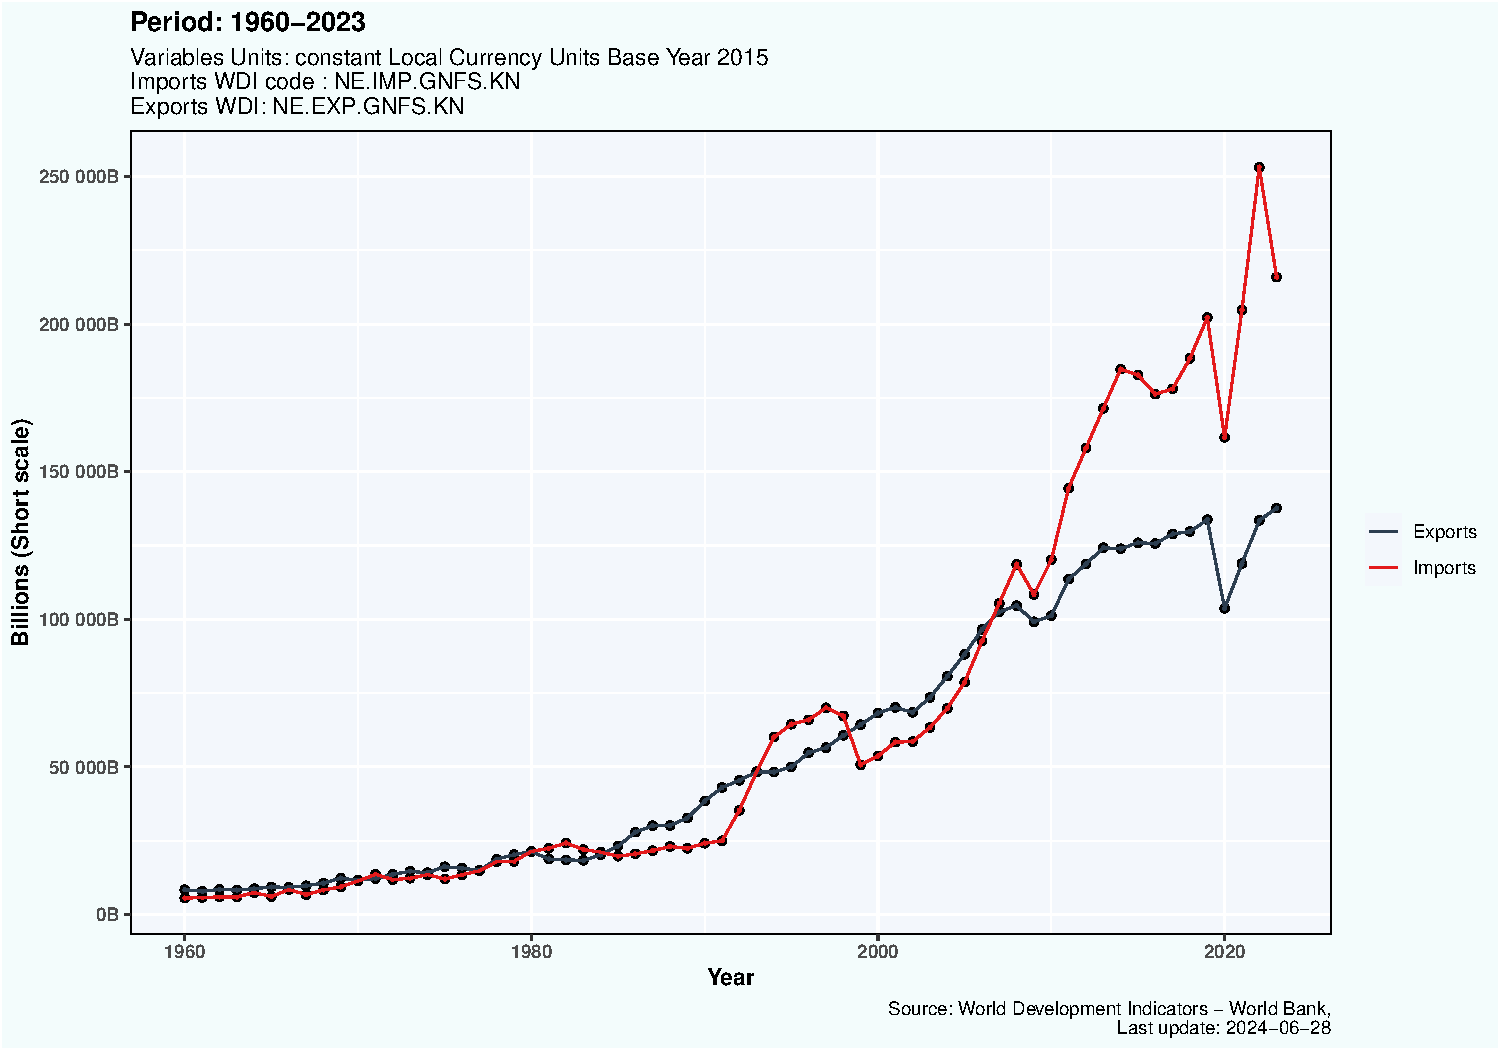
\includegraphics[width=0.85\textwidth,height=\textheight]{005_external_sector_II_files/figure-beamer/fig-imports-exports-col-1.pdf}

}

\caption{\label{fig-imports-exports-col}Colombia imports and exports}

\end{figure}%
\end{frame}

\section{Harmonized System (HS)}\label{harmonized-system-hs}

\begin{frame}{}
\phantomsection\label{section-5}
\begin{itemize}
\item
  The \textbf{Harmonized System (HS)} is a standardized numerical method
  of classifying traded goods that is internationally accepted and
  maintained by the \textbf{World Customs Organization (WCO)}
\item
  The HS code consists of 6-digits that are the same independent of the
  country:

  \begin{itemize}
  \tightlist
  \item
    First 2 digits designate the \textbf{HS} chapter
  \item
    Second 2 digits designate the \textbf{HS} heading
  \item
    Third 2 digits designate the \textbf{HS} subheading
  \end{itemize}
\item
  Example of \textbf{HS} code: 090111 (Coffee, not roasted, not
  decaffeinated)

  \begin{itemize}
  \tightlist
  \item
    Chapter \textbf{09}: Cofee, tea, mate and spices
  \item
    Heading \textbf{01}: Coffee, whether or not roasted or
    decaffeinated; coffee husks and skins; coffee substitutes containing
    coffee in any proportion
  \item
    Subheading \textbf{11}: Coffee, not roasted, not decaffeinated
  \end{itemize}
\end{itemize}
\end{frame}

\section{Patterns of international trade:
goods}\label{patterns-of-international-trade-goods}

\begin{frame}{}
\phantomsection\label{section-6}
\begin{figure}

\centering{

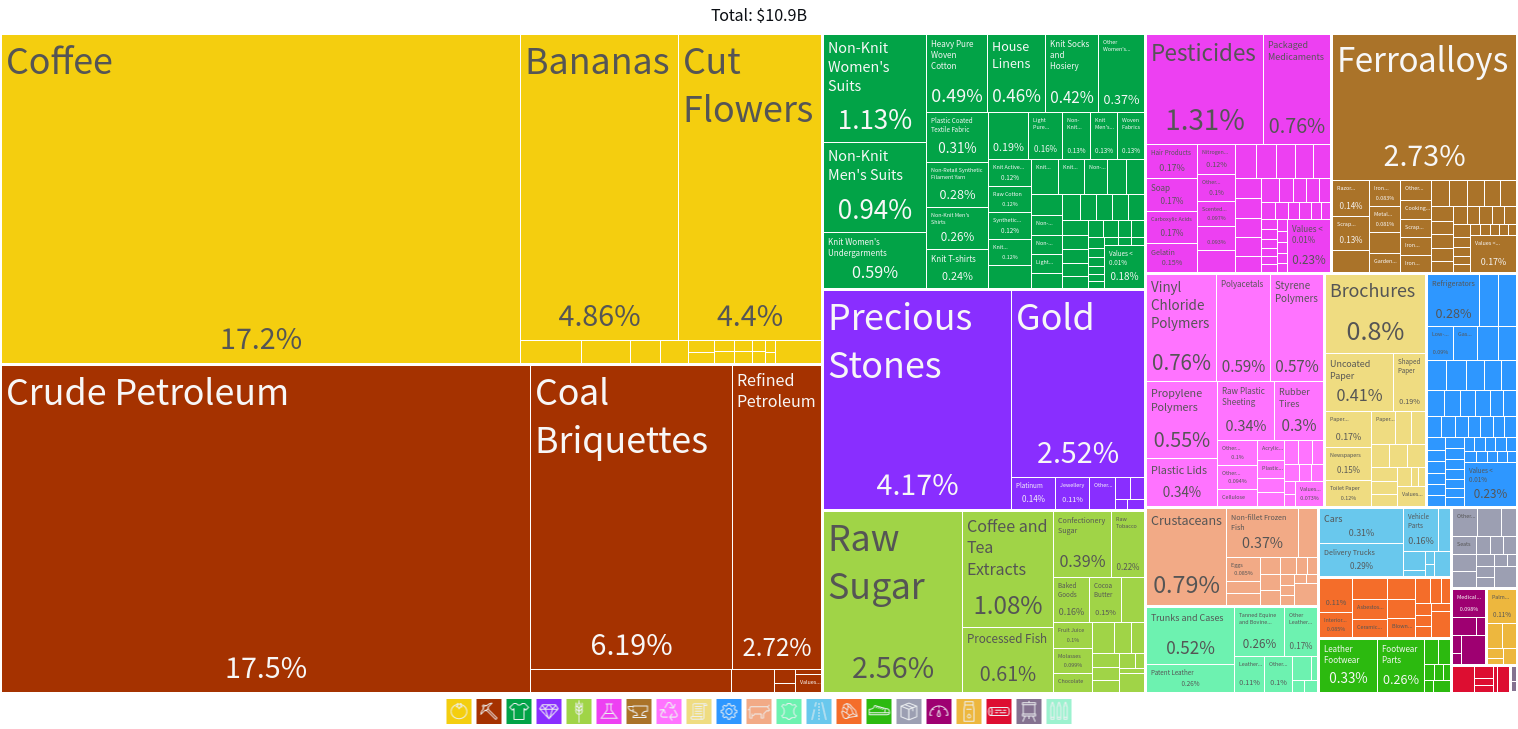
\includegraphics[width=4.6875in,height=4.6875in]{000_data/005_col_exports_1995_hs4_92.png}

}

\caption{\label{fig-colombian-goods-exports-1995}Colombian good exports
\textbf{HS 4 digits (HS92) edition} year 1995
(\citeproc{ref-oec_observatory_2022}{OEC 2022})}

\end{figure}%
\end{frame}

\begin{frame}{}
\phantomsection\label{section-7}
\begin{figure}

\centering{

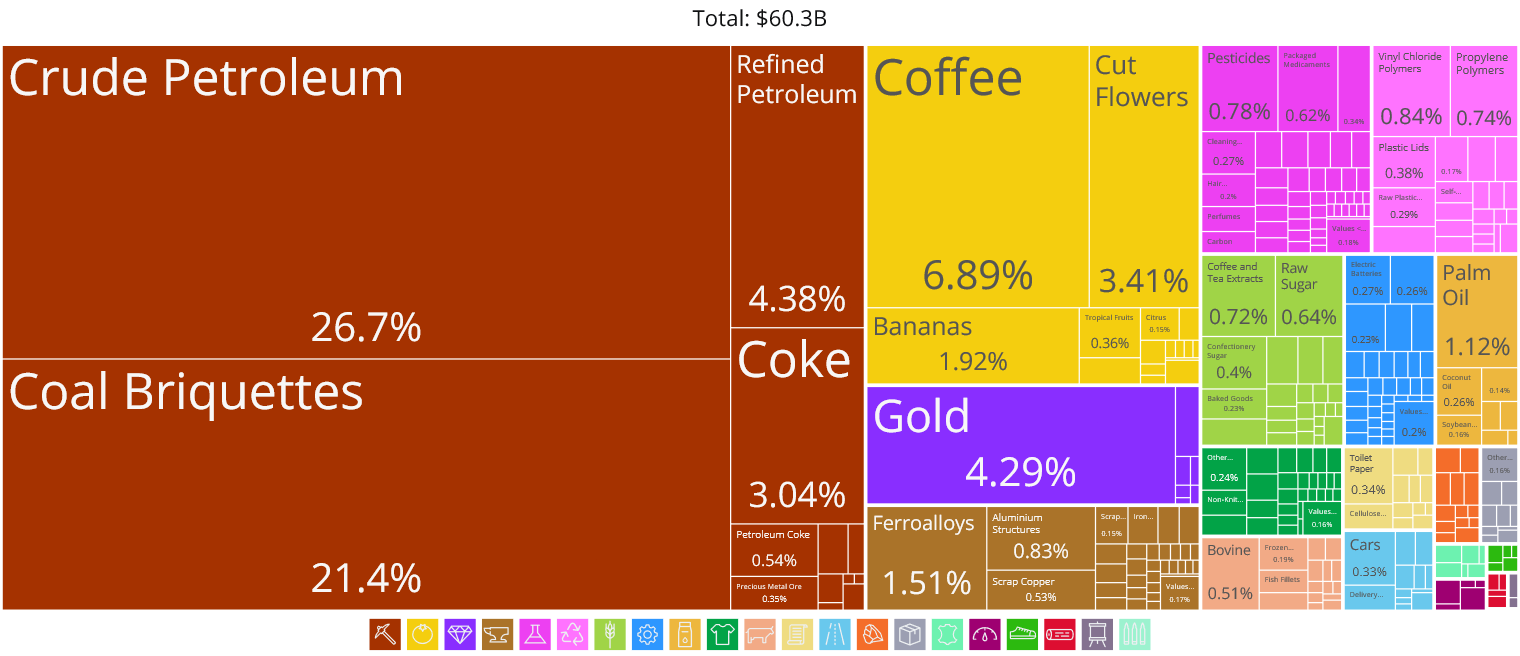
\includegraphics[width=4.6875in,height=4.6875in]{000_data/005_col_exports_2022_hs4_92.png}

}

\caption{\label{fig-colombian-goods-exports-2022}Colombian good exports
\textbf{HS 4 digits (HS92) edition} year 2022
(\citeproc{ref-oec_observatory_2022}{OEC 2022})}

\end{figure}%
\end{frame}

\begin{frame}{}
\phantomsection\label{section-8}
\begin{figure}

\centering{

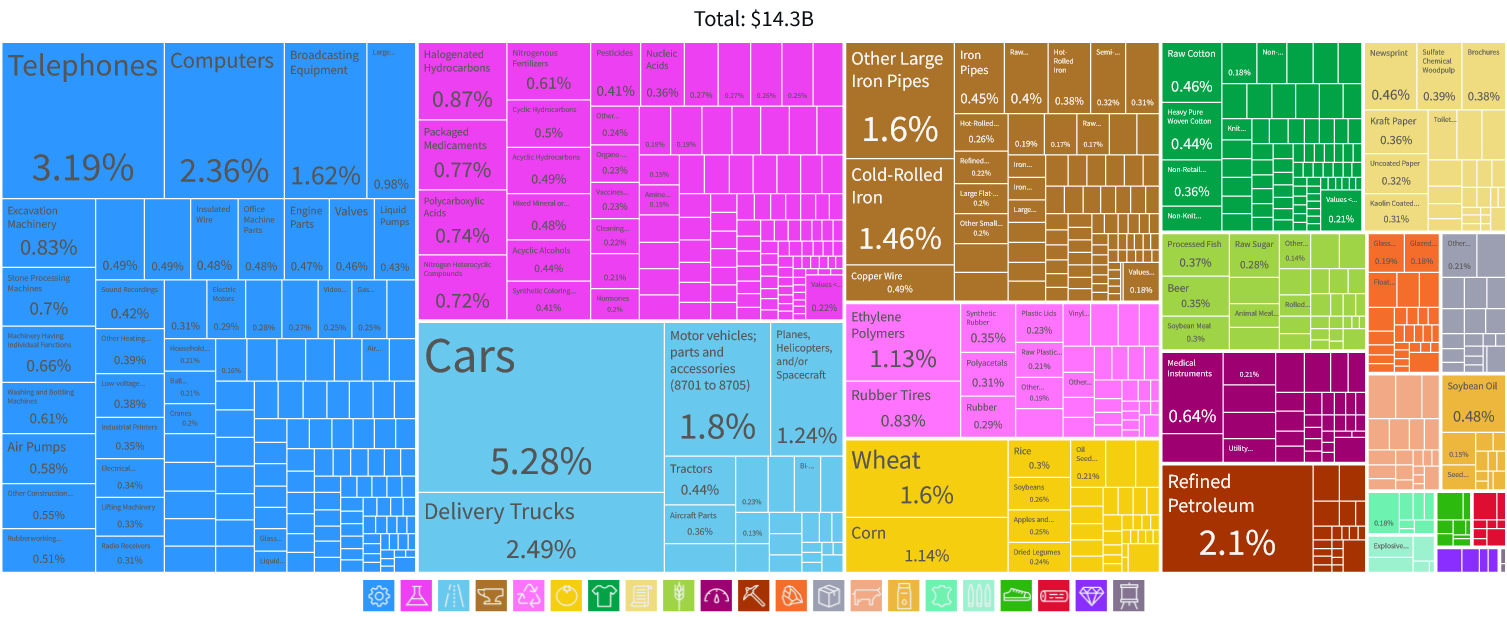
\includegraphics[width=4.6875in,height=4.6875in]{000_data/005_col_imports_1995_hs4_92.png}

}

\caption{\label{fig-colombian-goods-imports-1995}Colombian goods imports
\textbf{HS 4 digits (HS92) edition} year 1995
(\citeproc{ref-oec_observatory_2022}{OEC 2022})}

\end{figure}%
\end{frame}

\begin{frame}{}
\phantomsection\label{section-9}
\begin{figure}

\centering{

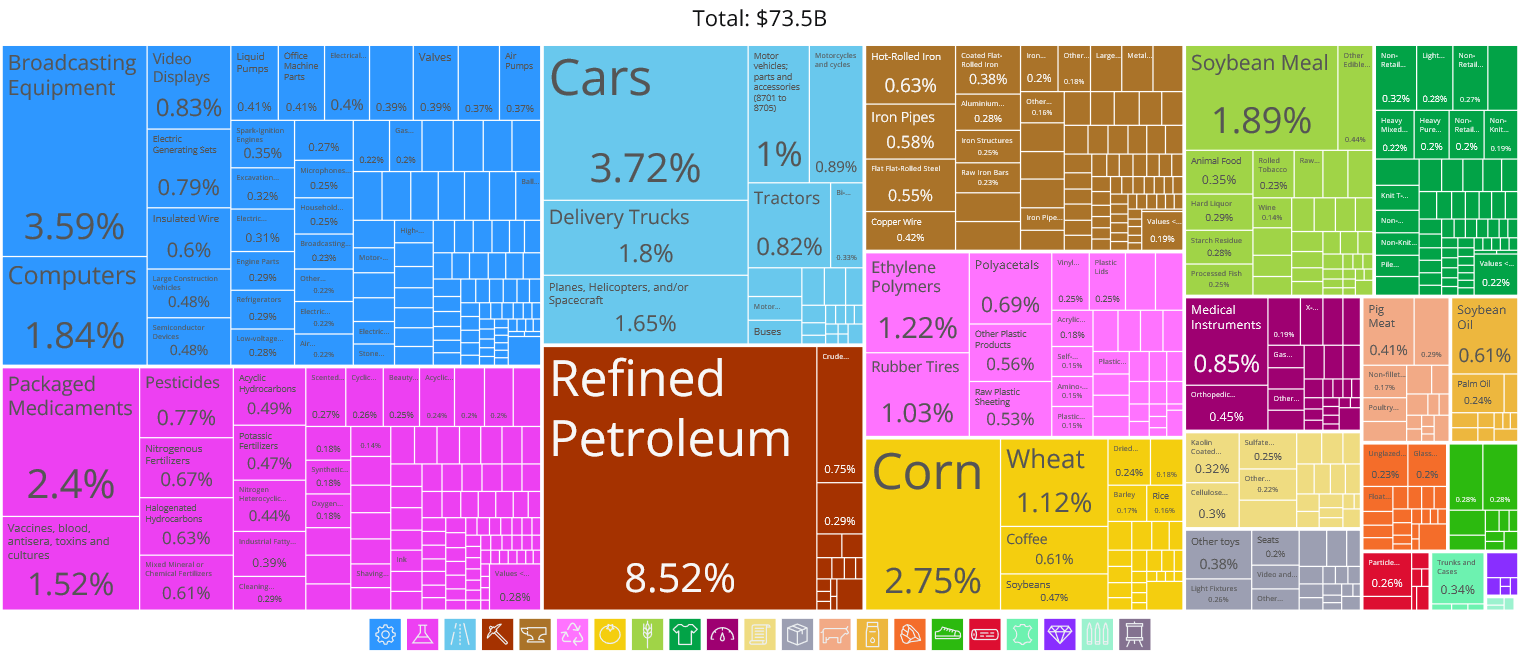
\includegraphics[width=4.6875in,height=4.6875in]{000_data/005_col_imports_2022_hs4_92.png}

}

\caption{\label{fig-colombian-goods-imports-2022}Colombian goods imports
\textbf{HS 4 digits (HS92) edition} year 2022
(\citeproc{ref-oec_observatory_2022}{OEC 2022})}

\end{figure}%
\end{frame}

\section{Extended Balance of Payments Services classification
(EBOPS)}\label{extended-balance-of-payments-services-classification-ebops}

\begin{frame}{}
\phantomsection\label{section-10}
\begin{itemize}
\item
  The EBOPS classification provides a breakdown of the Balance of
  Payments Trade in Services by types of services.
\item
  The classification thereby meets a number of user requirements,
  including the provision of more detailed information on Trade in
  services

  \begin{itemize}
  \tightlist
  \item
    \textbf{EBOPS 2002}
  \item
    \textbf{EBOPS 2010}
  \end{itemize}
\item
  For more information check out

  \begin{itemize}
  \tightlist
  \item
    (\citeproc{ref-vereinte_nationen_manual_2002}{Nationen and
    Kommission 2002})
  \item
    (\citeproc{ref-united_nations_manual_2012}{Nations 2012})
  \end{itemize}
\end{itemize}
\end{frame}

\section{Patterns of international trade:
services}\label{patterns-of-international-trade-services}

\begin{frame}{}
\phantomsection\label{section-11}
\begin{figure}

\centering{

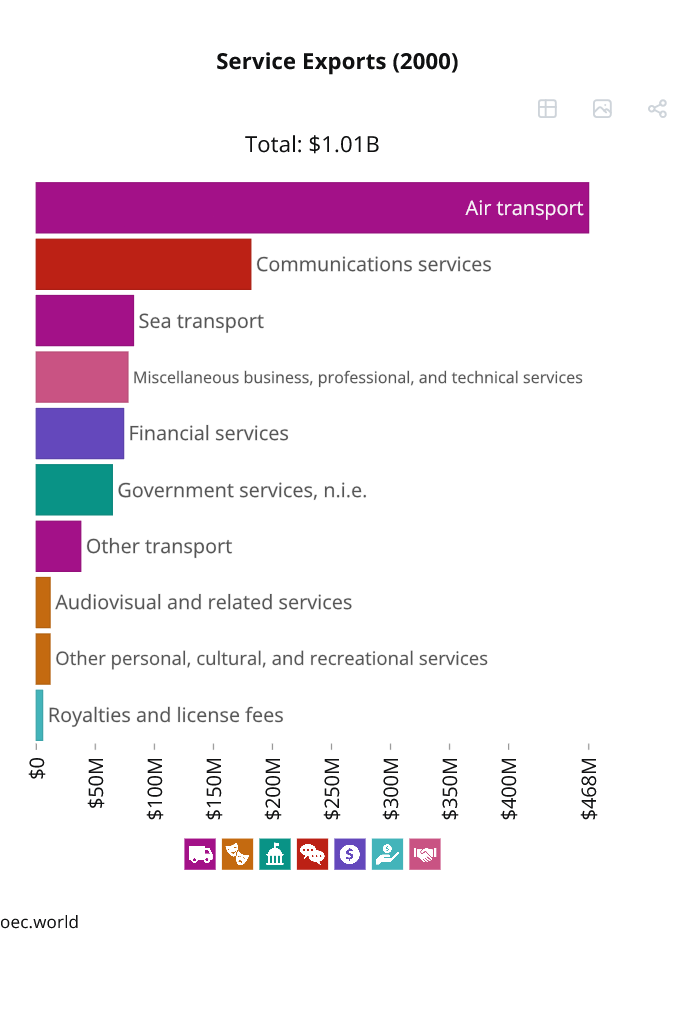
\includegraphics[width=2.91667in,height=2.91667in]{000_data/005_col_export_ebops_version2002_2000.png}

}

\caption{\label{fig-colombian-services-exports-2000}Colombian services
exports \textbf{(EBOPS Version 2002)} year 2000
(\citeproc{ref-oec_observatory_2022}{OEC 2022})}

\end{figure}%
\end{frame}

\begin{frame}{}
\phantomsection\label{section-12}
\begin{figure}

\centering{

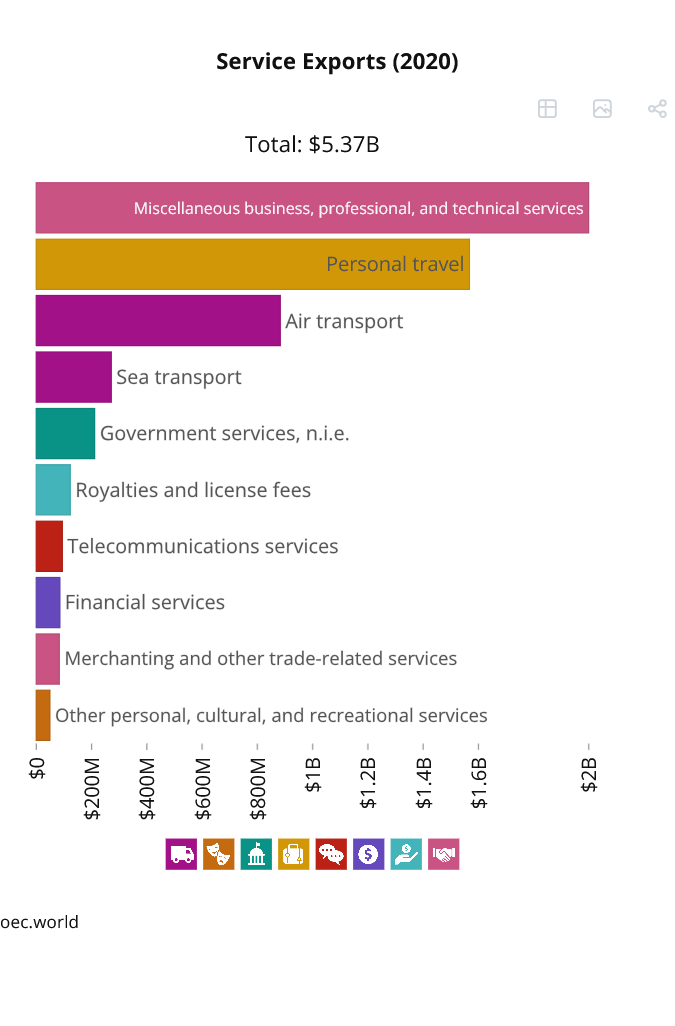
\includegraphics[width=2.60417in,height=2.60417in]{000_data/005_col_export_ebops_version2002_2020.png}

}

\caption{\label{fig-colombian-services-exports-2020}Colombian services
exports \textbf{(EBOPS Version 2002)} year 2020
(\citeproc{ref-oec_observatory_2022}{OEC 2022})}

\end{figure}%
\end{frame}

\begin{frame}{}
\phantomsection\label{section-13}
\begin{figure}

\centering{

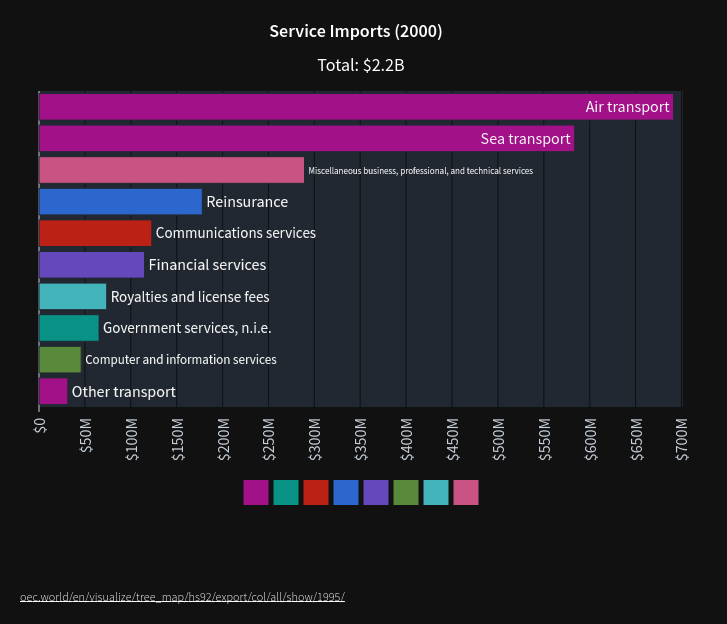
\includegraphics[width=2.91667in,height=2.91667in]{000_data/005_col_import_ebops_version2002_2000.png}

}

\caption{\label{fig-colombian-services-imports-2000}Colombian services
imports \textbf{(EBOPS Version 2002)} year 2000
(\citeproc{ref-oec_observatory_2022}{OEC 2022})}

\end{figure}%
\end{frame}

\begin{frame}{}
\phantomsection\label{section-14}
\begin{figure}

\centering{

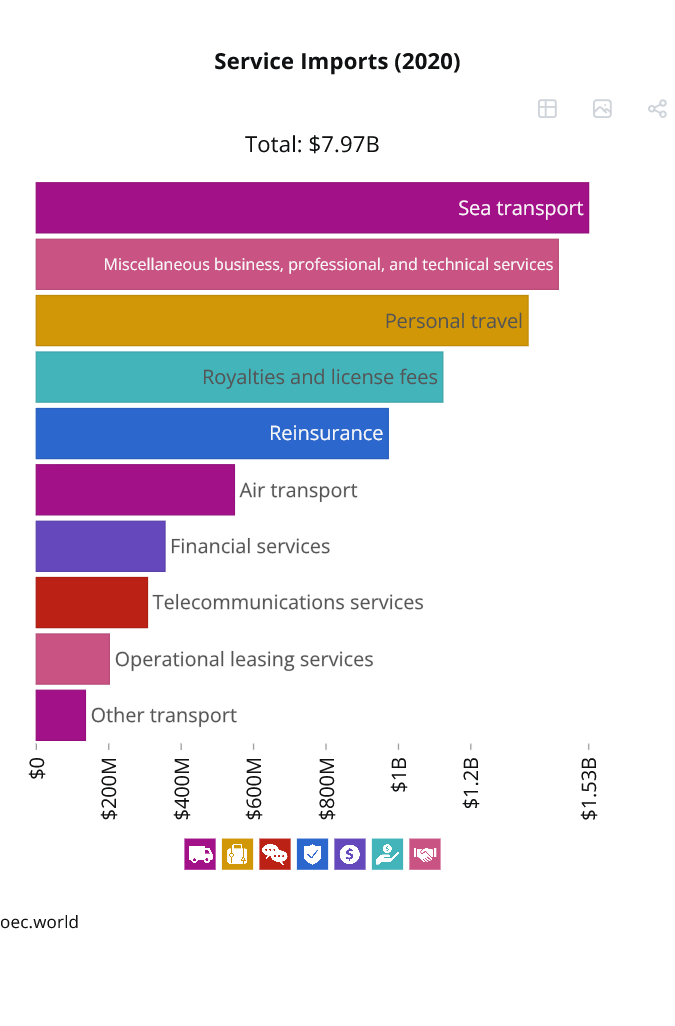
\includegraphics[width=2.60417in,height=2.60417in]{000_data/005_col_import_ebops_version2002_2020.png}

}

\caption{\label{fig-colombian-services-imports-2020}Colombian services
imports \textbf{(EBOPS Version 2002)} year 2020
(\citeproc{ref-oec_observatory_2022}{OEC 2022})}

\end{figure}%
\end{frame}

\section{Observatory of Economic Complexity
(OEC)}\label{observatory-of-economic-complexity-oec}

\begin{frame}{}
\phantomsection\label{section-15}
\begin{itemize}
\item
  \emph{``The Observatory of Economic Complexity (OEC) is an online data
  visualization and distribution platform focused on the geography and
  dynamics of economic activities''}
  (\citeproc{ref-oec_observatory_2022}{OEC 2022})
\item
  \emph{``The OEC is currently designed and developed by Datawheel, but
  it began as a research project at MIT's Collective Learning group
  (former Macro Connections Group)''}
  (\citeproc{ref-oec_observatory_2022}{OEC 2022})
\end{itemize}
\end{frame}

\begin{frame}{}
\phantomsection\label{section-16}
\begin{itemize}
\item
  Tree map

  \begin{itemize}
  \item
    \url{https://oec.world/} \textgreater{} TOOLS \textgreater{} Tree
    map

    \begin{itemize}
    \tightlist
    \item
      Country
    \item
      Product
    \item
      Bilateral
    \end{itemize}
  \end{itemize}
\item
  Profiles

  \begin{itemize}
  \tightlist
  \item
    \url{https://oec.world/} \textgreater{} PROFILES \textgreater{}
    Countries \textgreater{} Colombia
  \end{itemize}
\end{itemize}
\end{frame}

\section{Acknowledgments}\label{acknowledgments}

\begin{frame}{}
\phantomsection\label{section-17}
\begin{itemize}
\item
  To my family that supports me
\item
  To the taxpayers of Colombia and the
  \href{https://www.umng.edu.co/estudiante}{\textbf{UMNG students}} who
  pay my salary
\item
  To the \href{https://www.business-science.io/}{\textbf{Business
  Science}} and \href{https://www.rfordatasci.com/}{\textbf{R4DS Online
  Learning}} communities where I learn
  \href{https://www.r-project.org/about.html}{\textbf{R}} and
  \href{https://www.python.org/about/}{\textbf{\(\pi\)-thon}}
\item
  To the \href{https://www.r-project.org/contributors.html}{\textbf{R
  Core Team}}, the creators of
  \href{https://rstudio.com/products/rstudio/}{\textbf{RStudio IDE}},
  \href{https://quarto.org/}{\textbf{Quarto}} and the authors and
  maintainers of the packages
  \href{https://CRAN.R-project.org/package=tidyverse}{\textbf{tidyverse}},
  \href{https://CRAN.R-project.org/package=wbstats}{\textbf{wbstats}},
  \href{https://CRAN.R-project.org/package=tidyquant}{\textbf{tidyquant}},
  \href{https://CRAN.R-project.org/package=knitr}{\textbf{knitr}}, and
  \href{https://CRAN.R-project.org/package=tinytex}{\textbf{tinytex}}
  for allowing me to access these tools without paying for a license
\item
  To the \href{https://www.kernel.org/category/about.html}{\textbf{Linux
  kernel community}} for allowing me the possibility to use some
  \href{https://static.lwn.net/Distributions/}{\textbf{Linux
  distributions}} as my main
  \href{https://en.wikipedia.org/wiki/Operating_system}{\textbf{OS}}
  without paying for a license
\end{itemize}
\end{frame}

\section*{References}\label{references}
\addcontentsline{toc}{section}{References}

\begin{frame}[allowframebreaks]{References}
\phantomsection\label{refs}
\begin{CSLReferences}{1}{0}
\bibitem[\citeproctext]{ref-cardenas_introduccion_2020}
Cardenas, Mauricio. 2020. \emph{Introducción a La {Economía}
{Colombiana}}. 4th ed. Alfaomega.

\bibitem[\citeproctext]{ref-vereinte_nationen_manual_2002}
Nationen, Vereinte, and Europäische Kommission, eds. 2002. \emph{Manual
on Statistics of International Trade in Services}. Statistical Papers
{Series} {M} / {United} {Nations}, {Department} of {International}
{Economic} and {Social} {Affairs}, {Statistical} {Office} 86. Genf.

\bibitem[\citeproctext]{ref-united_nations_manual_2012}
Nations, United, ed. 2012. \emph{Manual on {Statistics} of
{International} {Trade} in {Services} 2010: {MSITS} 2010}. Rev. ed.
Economic \& {Social} {Affairs}. Geneva ; New York: United Nations.

\bibitem[\citeproctext]{ref-oec_observatory_2022}
OEC. 2022. {``The {Observatory} of {Economic} {Complexity} (5.1).''}
\url{https://oec.world/}.

\bibitem[\citeproctext]{ref-ridley_when_2010}
Ridley, Matt. 2010. {``When Ideas Have Sex.''}
\url{https://www.ted.com/talks/matt_ridley_when_ideas_have_sex?utm_campaign=tedspread&utm_medium=referral&utm_source=tedcomshare}.

\end{CSLReferences}
\end{frame}




\end{document}
